% Paper text converted from docs/paper.md. Page layout lives in preamble.tex; the author block is below.
% Preamble: document class, geometry, fonts, float and citation settings. The paper text in main.tex uses the macros below and plain LaTeX only.
\documentclass[10pt,twocolumn]{article}
\usepackage[T1]{fontenc}
\usepackage[utf8]{inputenc}
\usepackage{lmodern}
\usepackage[letterpaper,margin=0.75in,columnsep=0.25in]{geometry}
\usepackage{amsmath,amssymb}
\usepackage{graphicx}
\usepackage{booktabs}
\usepackage{array}
\usepackage{microtype}
\usepackage{enumitem}
\usepackage[hyphens]{url}
\Urlmuskip=0mu plus 1mu                    % allow line breaks inside long URLs in the reference list
\usepackage[authoryear,round]{natbib}      % author-year citations: \citet, \citep
\usepackage[hidelinks]{hyperref}
\bibliographystyle{plainnat}

% compact lists and floats
\setlist{nosep,leftmargin=*}
\setlist[itemize]{topsep=2pt}
\setlist[enumerate]{topsep=2pt}
\renewcommand{\topfraction}{0.9}
\renewcommand{\bottomfraction}{0.8}
\renewcommand{\textfraction}{0.1}
\renewcommand{\floatpagefraction}{0.8}
\renewcommand{\dbltopfraction}{0.9}
\renewcommand{\dblfloatpagefraction}{0.8}
\setcounter{topnumber}{3}
\setcounter{dbltopnumber}{3}
\setlength{\textfloatsep}{8pt plus 2pt minus 2pt}
\setlength{\dbltextfloatsep}{8pt plus 2pt minus 2pt}
\setlength{\intextsep}{6pt plus 2pt minus 2pt}
\setlength{\abovecaptionskip}{4pt}
\setlength{\belowcaptionskip}{0pt}
\usepackage[font=small,labelfont=bf,justification=raggedright]{caption}

% symbols used in the text
\newcommand{\qbar}{\ensuremath{\bar q}}
\newcommand{\phat}{\ensuremath{\hat p}}
\newcommand{\shat}{\ensuremath{\hat\sigma}}
\newcommand{\Stilde}{\ensuremath{\tilde S}}
\newcommand{\Atrain}{\ensuremath{A_{\mathrm{train}}}}
\newcommand{\Atest}{\ensuremath{A_{\mathrm{test}}}}

% headings never break a word across lines (same sizes as article's defaults)
\usepackage{titlesec}
\titleformat*{\section}{\Large\bfseries\raggedright\hyphenpenalty=10000 \exhyphenpenalty=10000 }
\titleformat*{\subsection}{\large\bfseries\raggedright\hyphenpenalty=10000 \exhyphenpenalty=10000 }

% reference list in small type with tight spacing
\renewcommand{\bibfont}{\footnotesize}
\setlength{\bibsep}{0pt plus 0.5pt}


\title{\bfseries Beyond $k$-Anonymity in Password Breach Checking:\\ How Robust Is Frequency-Smoothing Bucketization?}
\author{\begin{tabular}[t]{c@{\hspace{1.2em}}c@{\hspace{1.2em}}c}
Dilpreet Singh & Ishita Gupta & Madhav Raj\\
{\footnotesize National Institute of Technology Delhi} & {\footnotesize National Institute of Technology Delhi} & {\footnotesize National Institute of Technology Delhi}
\end{tabular}}  % author block: name with the institute in small font below (no emails or departments)
\date{}

\begin{document}
\maketitle

\begin{abstract}
Frequency-smoothing bucketization (FSB) lets a compromised-credential-checking server hide which leaked password a client is asking about, but its guarantee holds relative to the server's own estimate of the password distribution. We measure how far that guarantee carries when the estimate is noisy and the attacker holds the leak. Against the estimate-based attacker of Li et al.\ (CCS 2019), we reproduce FSB's result: at $q=\qbar=100$ guesses its loss over the no-bucket baseline is 0.0 percentage points (pp), against 41.1 pp for size-matched hash-prefix bucketization (HPB). That result tolerates multiplicative noise of about $\sigma=0.7$ on the estimate (5-point crossing; the head estimate we measure on held-out data has $\shat=0.31$). A count-aware attacker who ranks guesses by leak counts is stronger: FSB then loses 10.5 to 10.9 pp at $q=\qbar$, still about 73\% below HPB, but under a length-and-blocklist password policy it removes under 1\% of HPB's loss at $q=1$ for $\qbar=100$. The loss comes from rare passwords stored outside the estimate's histogram head, whereas HPB leaks popular head passwords. A larger head helps (2.3 pp at a 10M-entry head) but costs an estimated 77 MB of client data. A cold run of the attacker takes 14 s and 3.6 GB. Code and data-derivation scripts are public.
\end{abstract}

\section{Introduction}\label{sec:intro}

Compromised-credential checking (C3) services let a client find out whether a password appears in a breach corpus without sending it in the clear. Two services are widely used: Have I Been Pwned (HIBP) and Google Password Checkup. Both divide the leaked data into buckets, and the client reveals only the identifier of the bucket its credential would fall in, before running a private-set-intersection step inside that bucket. \citet[CCS][]{li2019} showed that revealing a hash prefix is not harmless: a server that sees the prefix can guess the password with far better odds than one that does not.

To reduce that leakage they proposed frequency-smoothing bucketization (FSB). FSB uses an estimate of the password distribution to assign popular passwords to several buckets, so that the bucket a client reveals is close to uniformly distributed given the password. Their simulations show that against an attacker who knows the same estimate, FSB leaks almost nothing at the guess budgets they study. The guarantee is therefore relative to the estimate the server uses, and two questions it leaves open decide whether FSB is safe to deploy.

\begin{itemize}
\item \textbf{How wrong can the estimate be?} The estimate is built from a leak and a language model, and no estimate matches the true distribution. How much error does FSB tolerate?
\item \textbf{How strong can the attacker be?} Li et al.\ give the attacker the full leak, but their simulated attacker ranks guesses with the server's estimate, and they note that this attack is not optimal. An attacker that ranks by the leak counts has not, to our knowledge, been measured. A real attacker may instead hold the leak, and so knows the counts of every stored password.
\end{itemize}

We answer both with a measurement study built on a 14M-password RockYou-based corpus. The server stores $N=13{,}125{,}513$ distinct passwords in $2^{24}$ buckets, and the estimate is a histogram head of the top $t=1{,}000{,}000$ passwords plus a character 3-gram tail. We compare FSB with size-matched HPB, giving HPB the larger bucket whenever the two cannot match exactly (up to 25\% larger), so any advantage we report for FSB is conservative.

Our contributions are five measurements.

\begin{enumerate}
\item \textbf{Reproduction (C1).} Against the estimate-based attacker, FSB's loss at $q=\qbar$ is 0.0 pp for $\qbar=10$, 100 and 1000, while size-matched HPB loses 37.0, 41.1 and 40.2 pp.
\item \textbf{Noise tolerance (C2).} Multiplying the estimate by a per-password lognormal factor, the loss reaches 5 pp at $\sigma=0.87$, 0.69 and 0.66 for $\qbar=10$, 100 and 1000. The error we measure on held-out data is $\shat=0.31$ for the head, so the margin is about two to one.
\item \textbf{A count-aware attacker (C3).} An attacker that weights guesses by leak counts and searches all 13.1M stored passwords gains 10.5, 10.9 and 10.9 pp at $q=\qbar$. That is still about 73\% less than HPB, but under a policy that rejects short and blocklisted passwords FSB removes less than 1\% of HPB's loss at $q=1$ for $\qbar=100$.
\item \textbf{Mechanism (C4).} FSB's residual loss is on rare passwords stored outside the histogram head (leak count 1 or 2 for 98.6\% of the targets gained at $q=1$), while HPB leaks the popular head passwords. Raising $t$ cuts the loss to 2.3 pp at 10M, but smoothing the 3-gram and calibrating the tail do not help, and noise confined to the tail does not move the count-aware attacker.
\item \textbf{Cost (C5).} The count-aware attacker needs 14 s and 3.6 GB for a cold run over all stored passwords.
\end{enumerate}

We also state what we did not measure: a leak larger than 14M passwords, usernames, generated guesses beyond the stored set, and a second corpus used as the leak. Section~\ref{sec:disc} lists them. Section~\ref{sec:bg} gives the protocols, Section~\ref{sec:setup} the threat model and setup, Section~\ref{sec:results} the results, and Sections~\ref{sec:related} and~\ref{sec:concl} related work and conclusions.

\section{Background}\label{sec:bg}

A C3 server holds a set $S$ of leaked passwords and publishes a bucketization: each stored password is assigned to one or more of $|B|$ buckets. To check a password $w$, the client picks a bucket that contains $w$, sends its identifier, and the two parties run a private-set-intersection protocol between $w$ and that bucket. The server learns the bucket identifier and nothing else, which is why the choice of bucket is the leakage we study. We follow Li et al.\ in treating the server as honest-but-curious and the protocol inside the bucket as ideal.

\textbf{Hash-prefix bucketization (HPB).} HIBP-style services assign $w$ to the bucket named by the first $l$ bits of its hash, so a bucket has about $|S|/2^l$ entries on average and each password lives in exactly one bucket. The bucket identifier is a deterministic function of $w$. A bucket therefore concentrates the probability mass of every popular password it contains, and a server that sees it can guess the most likely one.

\textbf{Frequency-smoothing bucketization (FSB).} FSB spreads popular passwords over many buckets so that a revealed bucket carries less information about which password produced it. Given an estimate $\phat$ of the password distribution and a target guess budget $\qbar$, let $w_{\bar q}$ be the $\qbar$-th most probable password under $\phat$. Password $w$ is stored in $\gamma(w)$ buckets and the client picks one of them uniformly at random:
\begin{equation*}
\gamma(w) = \min\left(|B|,\ \left\lceil |B| \cdot \frac{\hat p(w)}{\hat p(w_{\bar q})} \right\rceil\right)
\end{equation*}
Passwords at least as rare as $w_{\bar q}$ therefore sit in one or a few buckets, and the most popular passwords sit in many. Li et al.\ show that against an attacker who ranks guesses with the same $\phat$ and the true distribution equals $\phat$, a server seeing the bucket gains nothing over a server that sees nothing, as long as it makes at most $\qbar$ guesses. The price is bandwidth, because buckets grow.

\textbf{The estimate.} In practice $\phat$ comes from a leak. Following Li et al., our primary estimator stores the top $t=1{,}000{,}000$ passwords of the training leak by count as a histogram (the head) and scores every other string with a character 3-gram model with add-$\delta$ smoothing ($\delta=0.01$), rescaled so the tail mass is consistent with the head. We also evaluate a Kneser--Ney 3-gram and a cross-fitted isotonic calibration of the tail. Section~\ref{sec:intro} explains why we vary the estimate and the attacker, and Section~\ref{sec:results} what each variation shows.

\textbf{Guess budgets.} The attacker makes $q$ guesses after seeing the bucket. FSB's guarantee covers $q\le\qbar$. We report $q=1$, 10 and 100 for $\qbar=100$ and $q=\qbar$ for $\qbar\in\{10,100,1000\}$, and flag $q>\qbar$ separately because the guarantee does not extend there.

\section{Threat Model and Experimental Setup}\label{sec:setup}

\textbf{Threat model.} A C3 server, or anyone who reads its logs, sees the bucket identifier of a client's query and tries to guess the client's password within $q$ guesses. The attacker knows the bucketization, including the estimate $\phat$ and the bucket contents, and has no other side information about the target: we model password-only checking, as in HIBP and FSB, so there is no username. We measure the attacker's gain from the bucket, not its absolute success, because a no-bucket attacker already succeeds on common passwords.

\textbf{Data.} The leak is RockYou (14,326,970 unique passwords, 32,581,870 accounts after cleaning to printable ASCII of length 1 to 30). We split its accounts at random: 90\% form the training leak \Atrain, which the server stores as $\Stilde$ ($N=13{,}125{,}513$ unique passwords) and uses to build $\phat$, and the other 10\% form the target pool \Atest. phpbb (184,381 unique passwords, 255,417 accounts) serves as an out-of-distribution target pool. All splits use fixed seeds. The server has $2^{24}$ buckets, and the hash is a salted SHA-256 prefix.

\textbf{Attackers.} Both attackers see the bucket and rank its members to produce $q$ guesses; they differ in what they know.

\begin{itemize}
\item \textbf{est} weights each stored password by $\phat(w)/\gamma(w)$, the information Li et al.\ give the attacker. We run it over the 2M most probable stored passwords and check in Section~\ref{sec:c1} that using all of $\Stilde$ changes nothing for $q\le\qbar$.
\item \textbf{emp} weights each stored password by its leak count $/\ \gamma(w)$, as an attacker would who holds the same leak the server does. It searches all 13.1M stored passwords and generates no strings that are absent from the leak, so its results are lower bounds on what a stronger attacker could do. emp uses information that the threat model of Li et al.\ already grants the attacker (the leak) but that their simulations do not use. It is the headline attacker of this study.
\end{itemize}

\begin{figure*}[t]
\centering
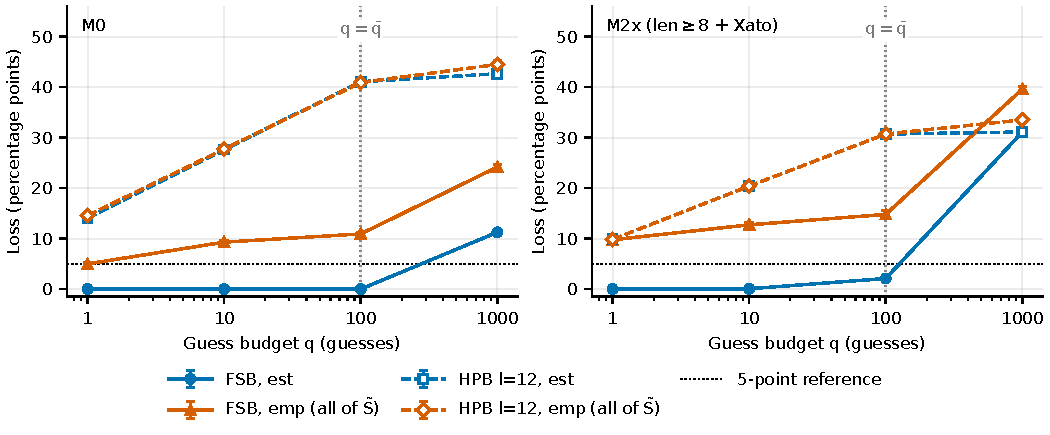
\includegraphics[width=\textwidth]{figs/fig1_wide.pdf}
\caption{Loss against guess budget $q$ (log scale) for M0 (a) and M2x (b): FSB with $\qbar=100$ and size-matched HPB with $l=12$ (average bucket 2,565 and 3,204 entries), against the est and emp attackers. Dotted vertical line: $q=\qbar$; dotted horizontal line: 5 pp. At $q=\qbar=100$ on M0: FSB est 0.00, FSB emp 10.92, HPB emp 40.90 pp; on M2x: FSB est 2.10, FSB emp 14.79, HPB emp 30.70 pp. Error bars: sd over 5 repeats of 5,000 targets.}
\label{fig:loss}
\end{figure*}

\textbf{Metric.} For each target we play the client's side (HPB: the bucket of the hash prefix; FSB: one of the $\gamma(w)$ buckets, uniformly) and let the attacker guess. Bucket success is the share of targets guessed within $q$ guesses. The baseline is the same attacker's success without a bucket, i.e.\ with its $q$ top candidates overall. The loss is bucket success minus baseline, in percentage points (pp). We use 5 repeats of 5,000 targets, drawn with replacement in proportion to leak count, and report the standard deviation over repeats. Targets that are not in $\Stilde$ can never be guessed, so they lower every success rate and add nothing to the loss.

\textbf{Size matching.} FSB with parameter $\qbar$ has an average bucket of 790, 2,565 and 11,336 entries for $\qbar=10$, 100 and 1000. We compare it with HPB at the nearest power-of-two prefix length ($l=14$, 12 and 10 bits), whose average buckets are 801, 3,204 and 12,818 entries. HPB therefore gets buckets that are 1\%, 25\% and 13\% larger, which favours HPB.

\textbf{Conditions.}

\begin{center}
\small
\renewcommand{\arraystretch}{1.1}
\setlength{\tabcolsep}{4pt}
\begin{tabular}{@{}>{\raggedright\arraybackslash}p{0.16\columnwidth}>{\raggedright\arraybackslash}p{0.27\columnwidth}>{\raggedright\arraybackslash}p{0.49\columnwidth}@{}}
\toprule
Condition & Targets & Server and attacker \\
\midrule
M0 (matched) & \Atest & $\phat$ and $\Stilde$ from \Atrain \\
M1b & phpbb accounts & as M0 (server estimate trained on RockYou only) \\
M2x (policy) & \Atest\ passwords with length $\geq 8$ and not on the Xato top-370 list & as M0; attacker candidates also restricted to policy-compliant passwords \\
M2L, M2B & policy ablations: length $\geq 8$ only, blocklist only & as M2x \\
M3 (noise) & \Atest & $\phat$ multiplied by $\exp(\sigma z_w)$, $z_w$ a fixed per-password standard normal; 5 independent draws; variants: all strings, tail only \\
\bottomrule
\end{tabular}
\end{center}

The policy conditions model a site that forbids weak passwords: the target distribution changes, but the server's data and the buckets do not. A further condition, in which the attacker is trained on a separate corpus, is saturated by confounds and is omitted (Section~\ref{sec:disc}).

\section{Results}\label{sec:results}

Unless stated otherwise $t=1{,}000{,}000$, the pool is \Atest, losses are in percentage points (pp) at $q=\qbar$, and $\pm$ is the standard deviation over 5 repeats of 5,000 targets.

\subsection{FSB holds against the estimate-based attacker (C1)}\label{sec:c1}

\begin{table*}[t]
\centering
\caption{Loss at $q=\qbar$ in pp (mean $\pm$ sd over 5 repeats). ``Removed'' is the share of the size-matched HPB loss that FSB removes (emp). ``Success ratio at $q=1$'' is the emp attacker's success at $q=1$ with the bucket divided by its success at $q=1$ without a bucket (mean $\pm$ sd over 5 repeats).}
\label{tab:headline}
\small
\setlength{\tabcolsep}{4.5pt}
\begin{tabular}{llrrrrrrr}
\toprule
Cond. & $\bar q$ & Avg.\ bucket & \multicolumn{3}{c}{Loss at $q=\bar q$ (pp)} & Removed & \multicolumn{2}{c}{Success ratio at $q=1$} \\
\cmidrule(lr){4-6}\cmidrule(lr){8-9}
 & & (entries) & FSB est & FSB emp & HPB emp & (\%) & FSB emp & HPB emp \\
\midrule
M0 & 10 & 790 & $0.00 \pm 0.00$ & $10.52 \pm 0.39$ & $37.09 \pm 0.56$ & $72$ & $7.0 \pm 1.4$ & $22.8 \pm 4.8$ \\
 & 100 & 2,565 & $0.00 \pm 0.00$ & $10.92 \pm 0.35$ & $40.90 \pm 0.65$ & $73$ & $6.2 \pm 1.1$ & $16.0 \pm 3.0$ \\
 & 1000 & 11,336 & $0.00 \pm 0.00$ & $10.91 \pm 0.35$ & $39.69 \pm 0.89$ & $73$ & $5.1 \pm 0.8$ & $10.2 \pm 1.9$ \\
\midrule
M1b & 10 & 790 & $0.00 \pm 0.00$ & $7.26 \pm 0.30$ & $31.10 \pm 0.38$ & $77$ & $3.8 \pm 0.9$ & $16.2 \pm 3.5$ \\
 & 100 & 2,565 & $0.00 \pm 0.00$ & $7.75 \pm 0.34$ & $35.12 \pm 0.51$ & $78$ & $3.3 \pm 0.9$ & $10.9 \pm 2.2$ \\
 & 1000 & 11,336 & $0.00 \pm 0.00$ & $7.62 \pm 0.28$ & $34.99 \pm 0.44$ & $78$ & $2.6 \pm 0.6$ & $6.8 \pm 1.2$ \\
\midrule
M2x & 10 & 790 & $0.96 \pm 0.09$ & $13.54 \pm 0.43$ & $27.82 \pm 0.35$ & $51$ & $87.9 \pm 24.4$ & $128.8 \pm 34.9$ \\
 & 100 & 2,565 & $2.10 \pm 0.24$ & $14.79 \pm 0.69$ & $30.70 \pm 0.40$ & $52$ & $85.1 \pm 24.6$ & $85.8 \pm 21.3$ \\
 & 1000 & 11,336 & $3.89 \pm 0.23$ & $16.59 \pm 0.35$ & $29.84 \pm 0.27$ & $44$ & $75.0 \pm 20.2$ & $53.2 \pm 11.2$ \\
\midrule
M2L & 10 & 790 & $0.38 \pm 0.10$ & $12.80 \pm 0.59$ & $28.15 \pm 0.59$ & $55$ & $18.7 \pm 4.3$ & $32.0 \pm 5.3$ \\
 & 100 & 2,565 & $1.66 \pm 0.03$ & $14.15 \pm 0.58$ & $30.36 \pm 0.62$ & $53$ & $17.7 \pm 4.1$ & $22.8 \pm 3.7$ \\
 & 1000 & 11,336 & $3.58 \pm 0.12$ & $16.07 \pm 0.41$ & $29.18 \pm 0.59$ & $45$ & $15.7 \pm 3.8$ & $15.7 \pm 2.7$ \\
\bottomrule
\end{tabular}

\end{table*}

With the est attacker, FSB loses 0.00 pp for every $q\le\qbar$ and every $\qbar\in\{10,100,1000\}$ on M0 and on the phpbb targets (M1b). Size-matched HPB loses 37.0, 41.1 and 40.2 pp at $q=\qbar$ on M0 and 31.5, 35.7 and 36.1 pp on M1b. At $q=1$, HPB's loss is 20.7, 14.1 and 8.4 pp for $\qbar=10$, 100 and 1000. Replacing the 2M candidate list with all 13.1M stored passwords does not change this for $q\le\qbar$, so the result is not an artefact of truncating the list. This reproduces the qualitative result of Li et al.\ on a different, smaller leak.

Two boundaries are visible in Figure~\ref{fig:loss}. First, the guarantee stops at $\qbar$: at $q=1000$ with $\qbar=100$ the FSB loss rises above 10 pp. Second, when targets follow a password policy that the estimate does not model (M2x), FSB's est loss is no longer zero: 0.96, 2.10 and 3.89 pp for $\qbar=10$, 100 and 1000, against 27.8, 30.7 and 28.8 pp for HPB. A likely cause is that the estimate assigns probability to passwords the policy forbids, so $\gamma$ is mis-set for those it allows; we did not isolate this. This agrees with the policy experiment of Li et al., who also find some loss at $q=100$ when the server's estimate ignores the policy.

\subsection{How much estimation error FSB tolerates (C2)}\label{sec:c2}

\begin{figure}[t]
\centering
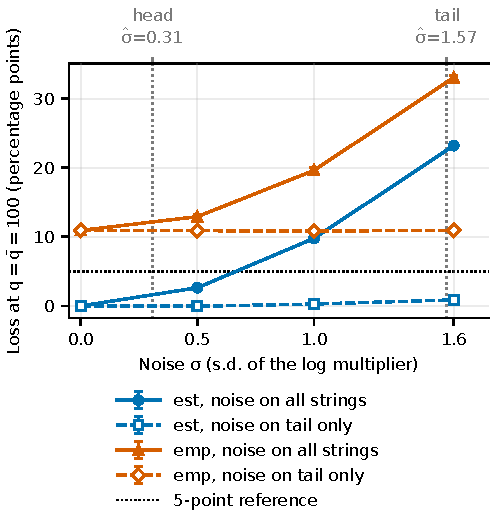
\includegraphics[width=\columnwidth]{figs/fig2.pdf}
\caption{Loss at $q=\qbar=100$ (M0, FSB) against the noise $\sigma$ that multiplies $\phat$ by $\exp(\sigma z_w)$, for noise on every string and on non-head (tail) strings only, est and emp. Points: mean over 5 independent noise draws, bars: sd over the draws; $\sigma=0$ is the noise-free run. Vertical dotted lines: measured $\shat$ on held-out data, head 0.308 and tail 1.570. Dotted horizontal line: 5 pp. Tail-only noise leaves emp at the clean-estimate loss of 10.92 pp (10.88 / 10.84 / 10.94 at $\sigma=0.5$ / 1.0 / 1.6); noise on every string raises it to 12.92 / 19.60 / 33.03. For est, tail-only noise gives $-0.04$ / $+0.28$ / $+0.89$ and full noise $+2.63$ / $+9.77$ / $+23.20$.}
\label{fig:noise}
\end{figure}

\begin{figure*}[t]
\centering
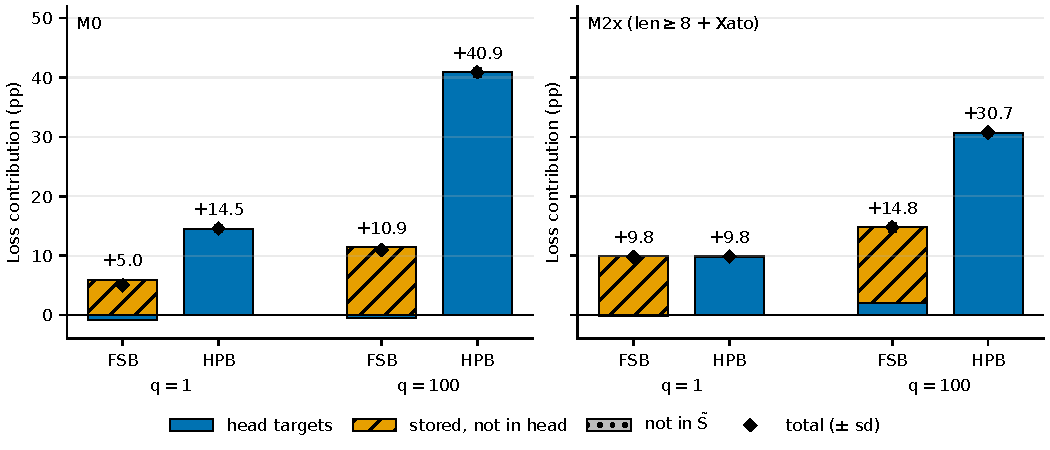
\includegraphics[width=\textwidth]{figs/fig3_wide.pdf}
\caption{Which targets the emp attacker gains on. Loss contribution = share of targets in the group $\times$ (attacker success $-$ baseline success) within the group; the contributions of the three groups add up to the loss (diamond, with sd over repeats; the number above each bar is the total, pp of all targets). Groups: head = top $t=1$M by leak count; stored, not in head = in $\Stilde$ but not in the head; not in $\Stilde$ = no candidate (contribution 0). FSB $\qbar=100$ and HPB $l=12$, $q=1$ and $q=100$, for M0 (a) and M2x (b). On M0 at $q=100$ the stored-not-in-head group contributes $+11.44$ of the FSB total $+10.92$ (head $-0.51$); under HPB the head group contributes $+40.90$ of $+40.90$.}
\label{fig:groups}
\end{figure*}

We multiply $\phat(w)$ by $\exp(\sigma z_w)$, where $z_w$ is a standard normal fixed per password by hashing, and rerun the est attacker. The loss at $q=\qbar$ reaches 5 pp at $\sigma=0.874\pm0.059$, $0.693\pm0.027$ and $0.658\pm0.013$ for $\qbar=10$, 100 and 1000 (mean and standard deviation over 5 independent draws of the noise). Smaller values of $\qbar$ tolerate more noise. The table in Appendix~\ref{app:noise} lists the per-draw crossings.

To place these thresholds, we measure the error of our own estimate on held-out data. Among passwords in the head, the log-ratio of true to estimated probability has a per-password dispersion $\shat=0.31$ (standard error 0.01 over 5 folds) and a bias of $-0.09$ log units. A coarser measurement that bins probability mass rather than passwords gives 0.11 and is a lower bound. The head error is therefore about half the 5-point threshold, and the margin of $\approx$ 2 to 1 is the main robustness result for FSB: the estimate has room to be wrong.

The error of the 3-gram tail is much larger, $\shat=1.57$ (0.92 by binned masses) with a bias of $+5.86$ log units, i.e.\ stored tail passwords are on average underestimated by a factor of about 350. This does not translate into loss for the est attacker. Putting noise on every string raises the loss at $q=\qbar=100$ to 2.63, 9.77 and 23.20 pp at $\sigma=0.5$, 1.0 and 1.6. Putting the same noise only on strings outside the head gives $-0.04$, 0.28 and 0.89 pp (Figure~\ref{fig:noise}). So the est attacker's loss is driven by head noise. The tail bias matters for a different attacker, as Section~\ref{sec:c4} shows.

\subsection{An attacker who holds the leak (C3)}\label{sec:c3}


The emp attacker ranks stored passwords by leak count instead of $\phat$ and searches all of $\Stilde$. On M0 it gains $10.52\pm0.39$, $10.92\pm0.35$ and $10.91\pm0.35$ pp against FSB at $q=\qbar$ for $\qbar=10$, 100 and 1000 (Table~\ref{tab:headline}). Against size-matched HPB it gains 37.1, 40.9 and 39.7 pp, so FSB still removes 72 to 73\% of the loss, and 77 to 78\% on the phpbb targets. The 2M-candidate version of the attacker gives lower numbers (Section~\ref{sec:disc}), so these are not upper bounds. At $q=1$ on M0 FSB's loss is 5.82, 4.99 and 3.97 pp against 21.10, 14.55 and 8.91 pp for HPB, i.e.\ FSB removes 72\%, 66\% and 55\%.

\textbf{A password policy erases the benefit at $q=1$.} Under M2x the popular passwords are gone, so the baseline attacker's success at $q=1$ falls from 0.97\% (M0) to 0.12\%. The bucket then lifts the emp attacker's $q=1$ success by a factor of $85\pm25$ under FSB and $86\pm21$ under HPB for $\qbar=100$, and the losses are 9.76 pp and 9.84 pp: FSB removes under 1\% of HPB's loss. For $\qbar=10$ the removal is 32\%. At $\qbar=1000$ the policy case is worse for FSB: at $q=1$ its loss is 8.58 pp against 6.06 pp for size-matched HPB, so FSB leaks more than HPB here (it removes $-41.7$\% of HPB's loss), even though HPB's buckets are 13\% larger at this $\qbar$ and favour HPB. The ratio rests on about six baseline successes per repeat, so we quote it only to show its order of magnitude. The length rule does most of this: with length $\geq 8$ alone (M2L) the emp loss at $q=\qbar$ is 12.8, 14.1 and 16.1 pp, and with the blocklist alone 3.4, 3.9 and 3.3 pp (2M-candidate lower bounds). At $\qbar=1000$ and $q=1$, FSB (7.90 pp) and HPB (7.88 pp) are indistinguishable on M2L.

\subsection{Where the loss comes from (C4)}\label{sec:c4}

\begin{figure}[t]
\centering
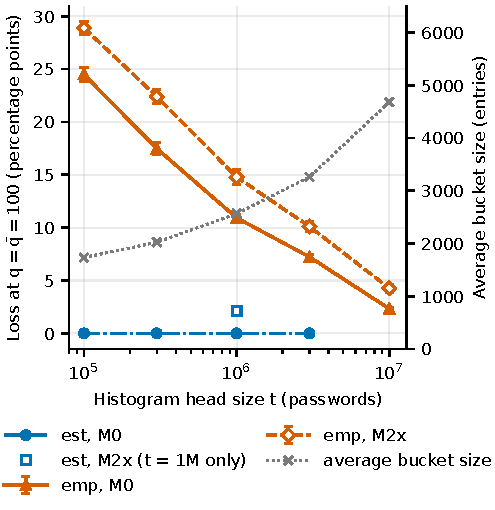
\includegraphics[width=\columnwidth]{figs/fig4.pdf}
\caption{emp loss at $q=\qbar=100$ (FSB $\qbar=100$) against the histogram head size $t$ (log scale), M0 (solid) and M2x (dashed); grey dotted curve, right axis: average bucket size. emp loss falls from 24.5 (M0) / 28.9 (M2x) at $t=100$k to 2.3 / 4.3 at $t=10$M. The est reference is not a flat zero everywhere: for M0 it is 0.00 at every $t$ that was measured (100k to 3M; not measured at 10M), while for M2x the only est measurement is at $t=1$M and is 2.10 pp (open square). Error bars: sd over 5 repeats of 5,000 targets.}
\label{fig:tsweep}
\end{figure}

We split the targets into three groups: the head (the top $t=1$M passwords by count in \Atrain; 50.8\% of the M0 targets), stored tail (in $\Stilde$ but outside the head; 11.7\%) and not in $\Stilde$ (37.5\%, never guessable). The loss splits as share $\times$ (success $-$ baseline) per group, and the three parts add up to the total (Figure~\ref{fig:groups}).

For FSB on M0 at $q=100$, the tail contributes $+11.44$ pp, the head $-0.51$ pp and the total is 10.92 pp. The attacker guesses 97.8\% of the stored tail targets and 8.1\% of the head targets. For HPB the pattern reverses: the head contributes all of the 40.90 pp (89.6\% of head targets guessed) and the tail nothing. At $q=1$ FSB's gain is again in the tail ($+5.90$ pp, 50.5\% of its targets guessed). Of the 1,476 targets that the attacker gains at $q=1$, 98.6\% have leak count 1 or 2, and their median $\gamma$ is 1. On M2x the story is the same: the tail contributes $+12.75$ of $+14.79$ pp.

We propose the following explanation. FSB flattens the posterior over the passwords it believes are popular, since $\phat(w)/\gamma(w)$ is roughly the same for all of them. A rare password that was nevertheless stored has $\gamma=1$ and a count of at least 1, so its posterior in its bucket exceeds that of any head password. The server's tail estimate puts such passwords far below that level, because they are underestimated by a factor of about 350 on average (Section~\ref{sec:c2}), and the est attacker inherits the mistake. The emp attacker has the counts and does not.

Three further measurements are consistent with this reading, though none proves it.

\begin{enumerate}
\item \textbf{A larger head shrinks the loss.} On M0 at $q=\qbar=100$ the loss is 24.5, 17.5, 10.9, 7.2 and 2.3 pp for $t=100$k, 300k, 1M, 3M and 10M (on M2x: 28.9, 22.4, 14.8, 10.1, 4.3). The average bucket also grows with $t$, from 1,733 to 4,682 entries, so the comparison holds $\qbar$ fixed and not the bucket size (Figure~\ref{fig:tsweep}).
\item \textbf{A better tail model should not help much.} Kneser--Ney and add-$\delta$ smoothing give the same loss at equal bucket size (for example 10.14 pp on M0 at $q=100$ and 6,500 entries, for both). A cross-fitted isotonic calibration of the tail, tuned on a held-out split and exploratory, helps by 0.0 to 0.8 pp at $q=100$ and by up to 2.3 pp at $q=1000$.
\item \textbf{Noise in the tail should leave the emp attacker unchanged.} With tail-only noise at $\sigma=0.5$, 1.0 and 1.6 its loss is 10.88, 10.84 and 10.94 pp, against 10.92 pp for the clean estimate. Noise on every string, which scrambles the head, raises it to 12.92, 19.60 and 33.03 pp (Figure~\ref{fig:noise}).
\end{enumerate}

\subsection{Cost of the attack and of a larger head (C5)}\label{sec:c5}

A cold run of the emp attacker over all 13,125,513 stored passwords takes 14.1 s and 3.57 GB, of which 8.6 s builds the index and 2.3 s plays the 25,000 bucket queries. With the 2M list it takes 4.9 s and 2.66 GB. The est attacker over all of $\Stilde$ needs 22.2 s and 3.63 GB. This is an attack that fits on a laptop.

The defender's side of the trade is a larger head. We estimate the storage of the head as the sum of string lengths plus one byte per entry, gzip-compressed, plus a 4-byte probability per entry (an estimate of data size, not an implementation). At $t=1$M the head covers 54.5\% of the training mass and takes 3.5 MB compressed text plus 4.0 MB of probabilities, 7.5 MB in total. At $t=10$M it covers 89.3\% and takes 36.9 MB plus 40 MB, 76.9 MB in total. The 3-gram table adds 3.6 MB (float32). Li et al.\ report an 8.9 MB estimate shipped as client code, which is of the same order as our 7.5 MB head plus 3.6 MB 3-gram table. The head at $t=10$M cuts the M0 loss to 2.3 pp but is about ten times the size of the $t=1$M head.

\section{Discussion and Limitations}\label{sec:disc}

\textbf{What the results say.} FSB's guarantee holds relative to the server's estimate, and against that attacker it has room for error: the head estimate can be roughly twice as noisy as ours before the loss reaches 5 pp. The guarantee does not hold against an attacker who holds the leak counts. That attacker still loses to FSB more than to HPB (72 to 73\% less loss on M0), so FSB is an improvement, but the loss it leaves is 10.5 to 10.9 pp at $q=\qbar$ and, under a length-and-blocklist password policy, FSB gives almost no protection at $q=1$ for $\qbar=100$, and at $\qbar=1000$ it is worse than size-matched HPB. We read this as a gap between the threat model and the estimate, not as a flaw in the smoothing idea: the loss sits on rare stored passwords that the estimate underrates by a factor of about 350.

\textbf{Design implications.} Three points follow from Section~\ref{sec:results}. A larger histogram head lowers the loss (2.3 pp at $t=10$M) at roughly ten times the storage of $t=1$M. Smoothing or calibrating the tail model barely changes it. A natural untested remedy is to bound $\gamma$ from below for stored tail passwords, so that a rare stored password is not the single likeliest guess in its bucket. We did not run it and do not claim it works.

\textbf{Limitations.} We list them because several of them could move the numbers.

\begin{itemize}
\item \textbf{One leak, one split.} The leak is RockYou (14.3M unique passwords) split once at random. It is much smaller than the corpora production services hold (Google's service covers over 4 billion credentials). Li et al.\ simulate on a leak of about 436 million passwords, so ours is about 3\% of that. The standard deviations we report come from re-sampling targets, not from re-splitting the leak.
\item \textbf{Small second corpus.} phpbb has 255,417 accounts, so M1b is a sanity check on out-of-distribution targets, not a precise measurement.
\item \textbf{The emp attacker only guesses stored passwords.} It generates no strings that are absent from the leak, and the 2M-candidate version is lower still, so all emp numbers are lower bounds on a stronger attacker.
\item \textbf{emp and the threat model of Li et al.} emp uses the leak counts. Li et al.\ grant the attacker the leak, so this is within their threat model, but an outside observer who sees only bucket identifiers may not have the counts.
\item \textbf{No usernames.} We model password-only checking, as HIBP and FSB do. Username-password schemes are outside this study.
\item \textbf{Noise model.} We model estimator error as independent lognormal noise per password. Real errors are likely correlated across similar passwords. The measured $\shat$ depends on the method (0.31 per password, 0.11 binned for the head), and the tail bias is partly selection: passwords that were stored are those that occurred.
\item \textbf{Explanations are partly inferred.} The mechanism in Section~\ref{sec:c4} fits three independent measurements, but we did not test an intervention such as a $\gamma$ floor.
\item \textbf{Calibration is exploratory.} It was tuned on a held-out split, and the fresh pool it was evaluated on shares passwords with that split.
\item \textbf{Policy conditions.} M1a, in which the attacker is trained on a separate corpus, is saturated and omitted. M2x applies the policy to targets and to attacker candidates but not to the server's estimate.
\item \textbf{Storage figures} are estimates of data size, not an implementation, and cover only the head and the 3-gram table, not transmission or update cost.
\end{itemize}

\section{Related Work}\label{sec:related}

\textbf{C3 services and protocols.} Troy Hunt's Pwned Passwords service, built with Cloudflare, has a client send only the first five characters of a SHA-1 hash and receive the matching bucket \citep{hunt}. Google's Password Checkup protocol checks username-password pairs, and its authors describe a cloud service covering over 4 billion breached credentials and report that 1.5\% of logins in their telemetry involve breached credentials \citep{thomas2019}. \citet{li2019} gave the first formal treatment of C3 services, showed that knowing the hash prefix can raise the efficacy of remote guessing attacks by a factor of 12 in some settings, and proposed FSB for password-only checking and an identifier-based bucketization for username-password pairs. They build the estimate from a histogram of the top $10^6$ passwords and a rescaled 3-gram model, simulate on a leak of about 436 million passwords, and report one experiment with a password policy that the estimate ignores, where FSB shows some loss at $q=100$ but still beats HPB. Our study takes their FSB as given and asks how it behaves outside the conditions of their evaluation. HIBP added padded responses in 2020 against passive response-size analysis \citep{ali2020}, and Microsoft's Password Monitor avoids bucketization with an OPRF and homomorphic encryption \citep{msr}.

\textbf{Credential tweaking and second-generation services.} Li et al.\ adapt the credential tweaking attack of \citet{pal2019}, which compromised more than 16\% of accounts in under 1,000 guesses, to the bucket setting. \citet{pal2022} then proposed Might I Get Pwned (MIGP), a second-generation service that also protects against tweaking and was deployed with Cloudflare. \citet{pasquini2024} analyse MIGP's leakage and propose MIGP 2.0 against breach extraction attacks, where an honest-but-curious client learns about stored credentials. That work studies leakage to a client of the stored data. We study leakage to the server of the client's password, and the question of how robust the first-generation password-only fix is.

\textbf{Position.} We are not aware of an earlier study that sweeps the estimation error of FSB or that measures an attacker who ranks guesses by leak counts; our literature search was not exhaustive.

\section{Conclusion}\label{sec:concl}

FSB does what it promises against the attacker it was designed for: zero loss for $q\le\qbar$, with a head estimate that can be about twice as noisy as ours. Against an attacker who holds the leak counts it leaves 10.5 to 10.9 pp of loss at $q=\qbar$ and, under a password policy, offers almost no protection at $q=1$ for $\qbar=100$. The loss comes from rare stored passwords, which the estimate underrates, and shrinks as the histogram head grows, at a storage cost we estimate at 77 MB for the 10M-entry head. Practitioners who deploy FSB should state its guarantee as relative to the estimate and size the head against an attacker with counts. Future work should test a floor on $\gamma$ for tail passwords, repeat the study on a larger leak and a second corpus used as the leak, and give the attacker generated guesses.

\textbf{Ethics.} We use publicly available leaked password corpora (RockYou and phpbb, via SecLists) and simulate the server and the attacker on held-out accounts. We contacted no service, and no real account or live C3 query was involved. The attacker we describe needs only the leak and a laptop, so we report its cost to let defenders size their parameters.

\textbf{Use of generative AI.} Generative AI tools were used to help write the code and drafts of this paper. The authors reviewed the code and results and take responsibility for the content; all numbers are generated from the result files by scripts in the repository.

\textbf{Availability.} Code, result files and the scripts that regenerate every figure, table and number are at \url{github.com/dilpreet579/fsb-robustness-isp-paper}.

% References 7 (Kneser and Ney) and 8 (SecLists) appear in the md reference list but are not cited in the md text; kept in the list without changing the text.
\nocite{kneser1995,miessler}
\bibliography{refs}

\appendix
\onecolumn  % appendix is set full width so that its wide table and figure need no float tricks

\section{Per-draw noise crossings}\label{app:noise}

\begin{table}[h]
\centering
\caption{Sigma at which the est loss at $q=\qbar$ reaches 5 pp, for each of the five noise draws (M3, noise on all strings).}
\label{tab:noise}
\small
\begin{tabular}{lrl}
\toprule
$\bar q$ & $\sigma$ at 5 points (mean $\pm$ sd, 5 draws) & Per-draw values \\
\midrule
10 & $0.874 \pm 0.059$ & 0.940, 0.878, 0.913, 0.851, 0.788 \\
100 & $0.693 \pm 0.027$ & 0.661, 0.731, 0.708, 0.687, 0.677 \\
1000 & $0.658 \pm 0.013$ & 0.653, 0.665, 0.675, 0.651, 0.643 \\
\midrule
\multicolumn{3}{p{0.92\linewidth}}{\footnotesize emp (all of $\tilde S$): crossing not defined, the loss at $\sigma=0$ already exceeds 5 points (10.5 / 10.9 / 10.9 pp for $\bar q=10/100/1000$).} \\
\bottomrule
\end{tabular}

\end{table}

For the emp attacker (all of $\Stilde$) no crossing exists, because its loss at $\sigma=0$ already exceeds 5 pp (10.5, 10.9 and 10.9 pp).

\section{Head storage}\label{app:head}

\begin{table}[h]
\centering
\caption{Head size $t$, estimated head storage and emp loss (FSB $\qbar=100$, M0 and M2x).}
\label{tab:head}
\small
\setlength{\tabcolsep}{3pt}
\begin{tabular}{rrrrrrrrrrr}
\toprule
$t$ & \multicolumn{3}{c}{Head storage (MB)} & Avg.\ bucket & \multicolumn{3}{c}{emp loss, M0 (pp)} & \multicolumn{3}{c}{emp loss, M2x (pp)} \\
\cmidrule(lr){2-4}\cmidrule(lr){6-8}\cmidrule(lr){9-11}
 & text & gzip & +probs & (entries) & $q{=}1$ & $q{=}10$ & $q{=}100$ & $q{=}1$ & $q{=}10$ & $q{=}100$ \\
\midrule
100\,000 & 0.8 & 0.4 & 0.4 & 1,733 & $11.5 \pm 0.2$ & $20.5 \pm 0.5$ & $24.5 \pm 0.6$ & $20.1 \pm 0.4$ & $25.9 \pm 0.6$ & $28.9 \pm 0.6$ \\
300\,000 & 2.5 & 1.1 & 1.2 & 2,023 & $8.1 \pm 0.3$ & $14.9 \pm 0.3$ & $17.5 \pm 0.6$ & $15.1 \pm 0.4$ & $19.5 \pm 0.6$ & $22.4 \pm 0.6$ \\
1\,000\,000 & 8.5 & 3.5 & 4.0 & 2,565 & $5.0 \pm 0.3$ & $9.3 \pm 0.3$ & $10.9 \pm 0.3$ & $9.8 \pm 0.4$ & $12.7 \pm 0.5$ & $14.8 \pm 0.7$ \\
3\,000\,000 & 27.9 & 10.6 & 12.0 & 3,262 & $3.2 \pm 0.1$ & $6.3 \pm 0.2$ & $7.2 \pm 0.3$ & $6.5 \pm 0.1$ & $8.3 \pm 0.4$ & $10.1 \pm 0.5$ \\
10\,000\,000 & 96.2 & 36.9 & 40.0 & 4,682 & $1.5 \pm 0.1$ & $2.2 \pm 0.1$ & $2.3 \pm 0.2$ & $2.6 \pm 0.2$ & $2.8 \pm 0.2$ & $4.3 \pm 0.4$ \\
\bottomrule
\end{tabular}


\vspace{4pt}
\begin{minipage}{0.95\textwidth}\footnotesize
Storage is an estimate of data size, not an implementation: newline-delimited head strings (text), the same text under gzip -9, and 4 bytes per entry for a float32 probability (+probs); 1 MB = $10^6$ bytes. The 3-gram table adds 3.6 MB (float32) or 7.2 MB (float64). FSB with $\bar q=100$, emp attacker holding all of $\tilde S$.

\end{minipage}
\end{table}

\section{Fixes at equal bucket size}\label{app:fix}

\begin{figure}[h]
\centering
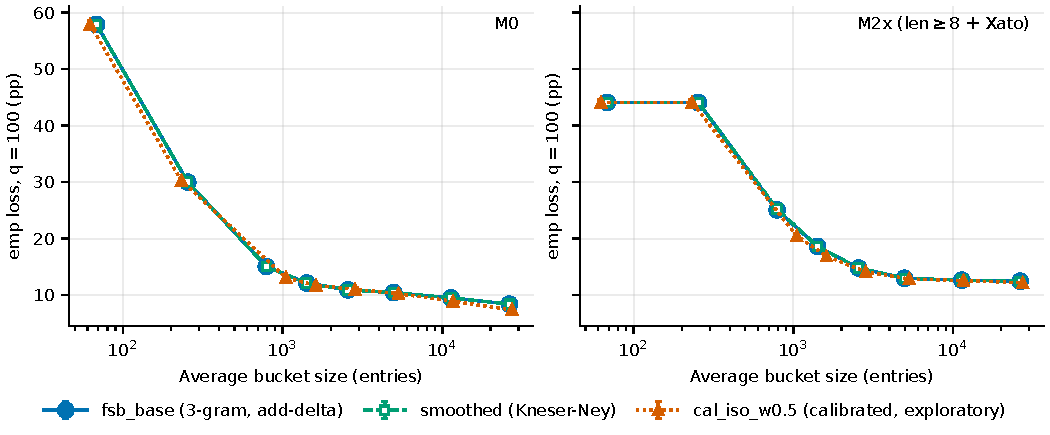
\includegraphics[width=\textwidth]{figs/fig5_wide.pdf}
\caption{emp loss at $q=100$ against the average bucket size (log scale) along a $\qbar$ sweep of 1 to 3000, for the base 3-gram (add-$\delta$), the Kneser--Ney 3-gram, and the calibrated tail estimate (exploratory: cross-fitted isotonic calibration of the tail, 0.5-decade bins), M0 (a) and M2x (b). The base and Kneser--Ney curves coincide (the base is drawn with larger markers underneath).}
\label{fig:fix}
\end{figure}

\end{document}
